\section{Hands-On Preparation Plan}

This plan is our recommendation and an assumption. Documentation facts that support single steps carry citations.

\paragraph{Lab environment.}
Use a disposable local virtual machine with Ubuntu Server 24.04 LTS. We chose Ubuntu because the guides we cite for SSH and Docker are Ubuntu guides, and because Google's own workstation distribution was based on Ubuntu until 2018 \cite{google-cloud-blog} (Section~\ref{sec:os}). Debian, the base of that distribution since 2018, would also work. Start with 2~vCPUs, 4~GB of RAM and 40~GB of disk, on a host with at least 8~GB of RAM. The RAM and disk figures are above the Section~\ref{sec:hardware} minimums, to leave room for containers, and the CPU figure equals the minikube minimum. Complete the installation, the package updates, and the user, permission and network configuration. SSH supports key authentication instead of a password \cite{ubuntu-server-docs-how-to-security-openssh-server}, so finish this step with an SSH key login. Then add Git with Bash or Python, Docker Engine and Prometheus, in this order. Add minikube and kubectl only after the core lab passes \cite{minikube-sigs-k8s-docs-start}.

\paragraph{Roadmap with completion gates.}
Advance to the next gate only when the current gate passes.
\begin{enumerate}
  \item Show an SSH login to the lab, and inspect processes, memory, files and sockets.
  \item Keep a small HTTP service and a Bash or Python health-check script in Git, and test healthy and failed responses. A Git commit records a snapshot that can later be reverted to or compared \cite{git-scm-book-en-v2-git-basics-recording-changes-to-the-repository}.
  \item Containerize the service, and show a reproducible startup, an HTTP request and the logs. Docker's Ubuntu guide verifies an installation by running the hello-world image \cite{docs-docker-engine-install-ubuntu}.
  \item Scrape the service metrics with Prometheus, which collects metrics from HTTP endpoints \cite{prometheus-docs-prometheus-latest-getting-started}. Record the four golden signals \cite{sre-book} and test a documented practice alert.
  \item Stop the service or introduce a permission error. Document detection, evidence, mitigation and recovery, and write a postmortem with impact, timeline, contributing causes and a preventive action. The SRE book recommends regular review sessions for postmortem drafts \cite{sre-book}.
\end{enumerate}
As an optional extension, deploy the same service to a local minikube cluster and reproduce a configuration change and a recovery.

\paragraph{Deliverables.}
Keep a reproducible README, the versioned lab configuration, the health-check script, the monitoring evidence and a reviewed postmortem. Ask a peer to reproduce the setup and review the incident explanation. The SRE Workbook cautions that automation should not remove human understanding of what is going wrong \cite{workbook}.

\begin{figure}[!b]
\centering
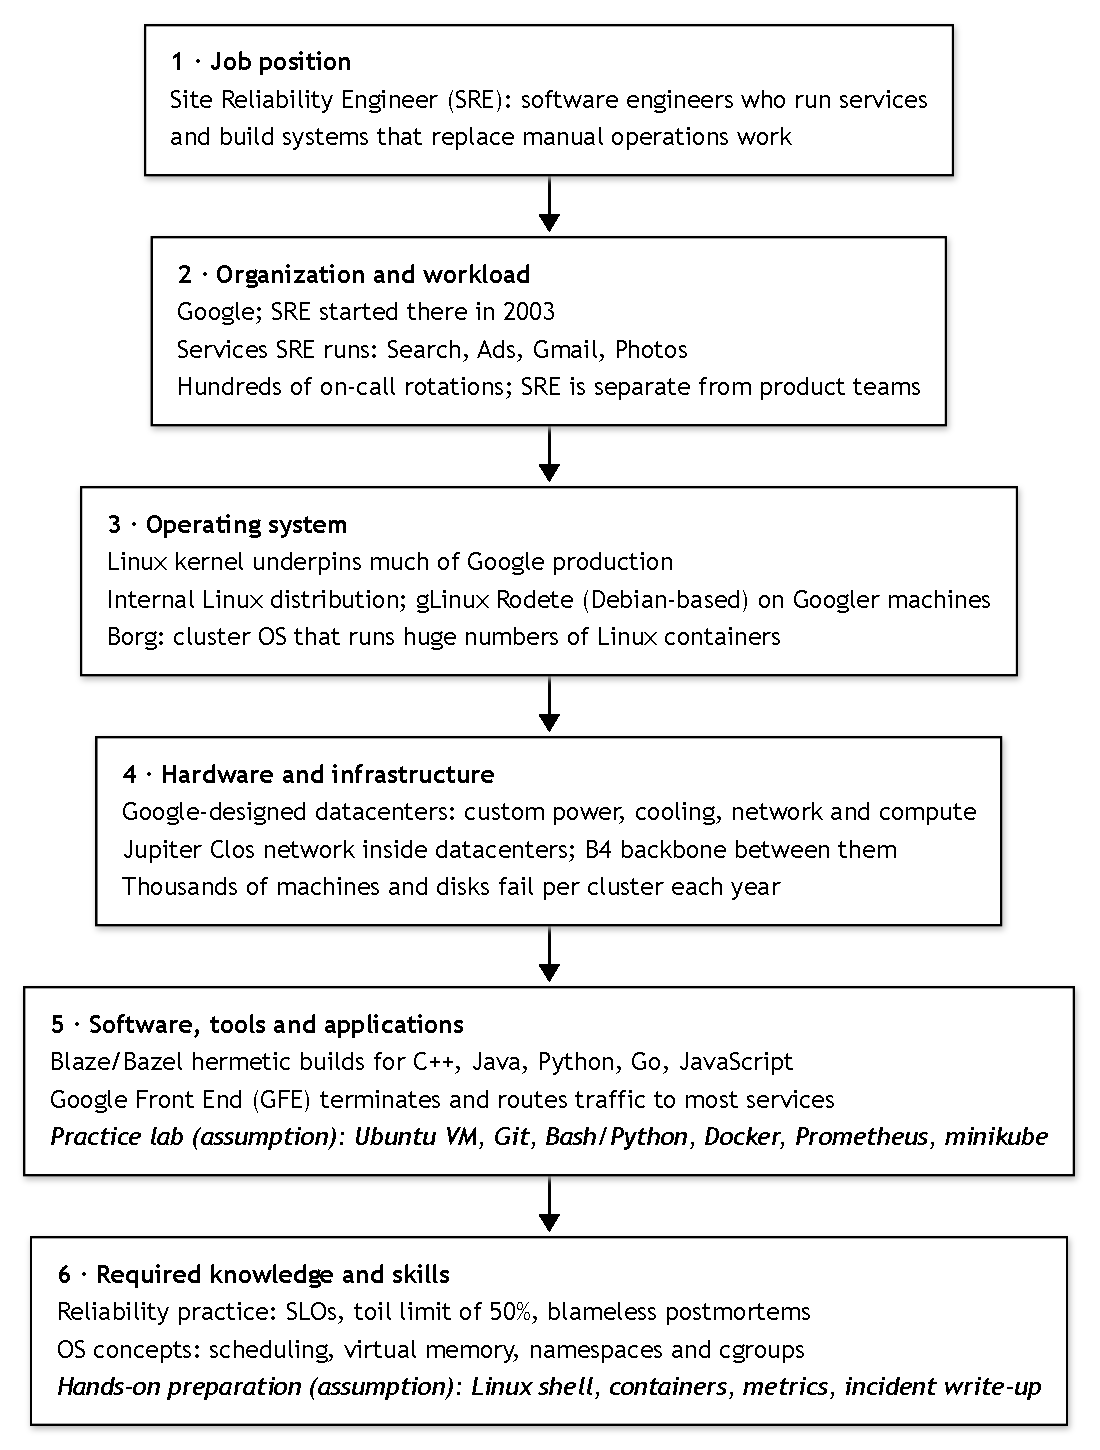
\includegraphics[width=0.94\textwidth,height=0.60\textheight,keepaspectratio]{figures/relationship.pdf}
\caption{From job position to required knowledge and skills for an SRE at Google. Most sources date from 2017 to 2020. Each stage rests on claims from the cited sources \cite{sre-book,workbook,bsrs,google-cloud-blog,static-pdf-incidentmanagementguide-pdf,man7,kernel-docs}. The arrows read: works at, runs on, sits on top of, is operated with, requires. The two italic lines are our assumptions, a typical practice environment and a preparation recommendation, not verified facts about Google. The link from the OS concepts to the job is our interpretation.}
\label{fig:chain}
\end{figure}
